\section{Appendix}
The code can be found at: \url{https://github.com/MelissaJessen/Shallow-Water-Equations}.



\subsection{FNO Toro test 1}
To test the FNO model on a more challenging problem, we consider the Toro test case 1.
We use the same model as before, but we train it on the data from the Toro test case 1.
Again, we use the first $80\%$ of the data for training and the last $20\%$ for testing.
The results of the model are shown in \autoref{fig:FNO_Toro_test1_predictions_3D} and \autoref{fig:FNO_Toro_test1_predictions}.

\begin{figure}[H]
    \centering
    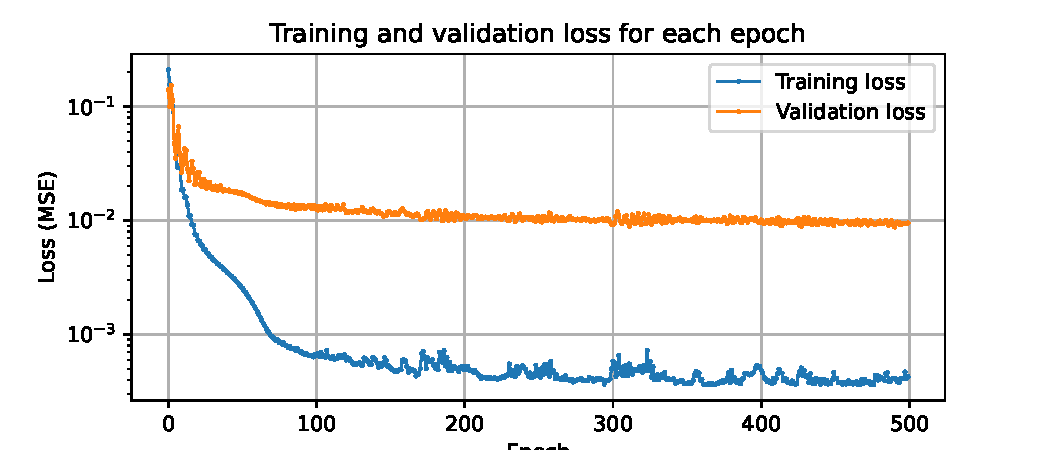
\includegraphics[width=0.7\textwidth]{C:/Users/Matteo/Shallow-Water-Equations/plots/torotest1_loss.pdf}
    \caption{FNO Toro test 1 loss.}\label{fig:FNO_Toro_test1_loss}
\end{figure}

\begin{figure}[H]
    \centering
    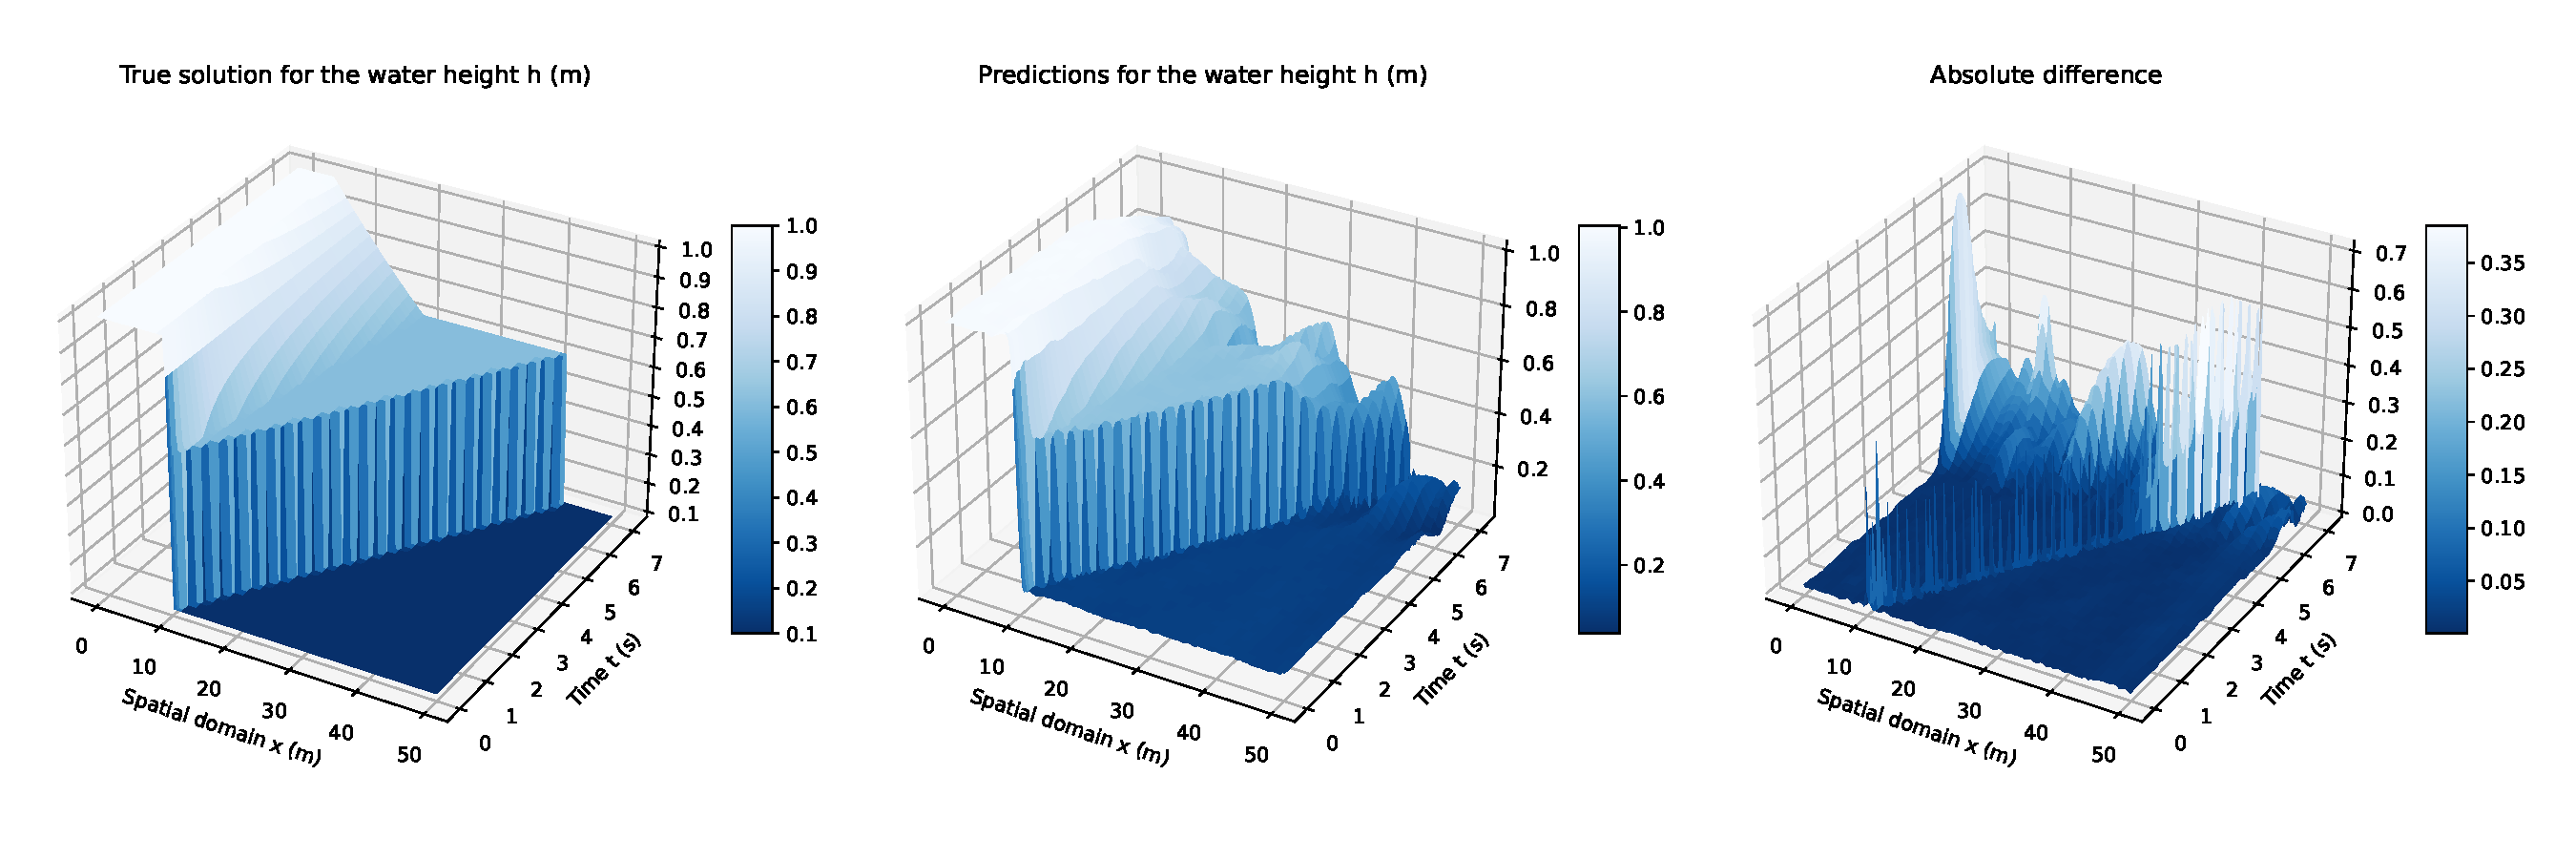
\includegraphics[width=0.9\textwidth]{C:/Users/Matteo/Shallow-Water-Equations/plots/torotest1_predictions_3D.pdf}
    \caption{FNO Toro test 1 predictions in 3d.}\label{fig:FNO_Toro_test1_predictions_3D}
\end{figure}


\begin{figure}[H]
    \centering
    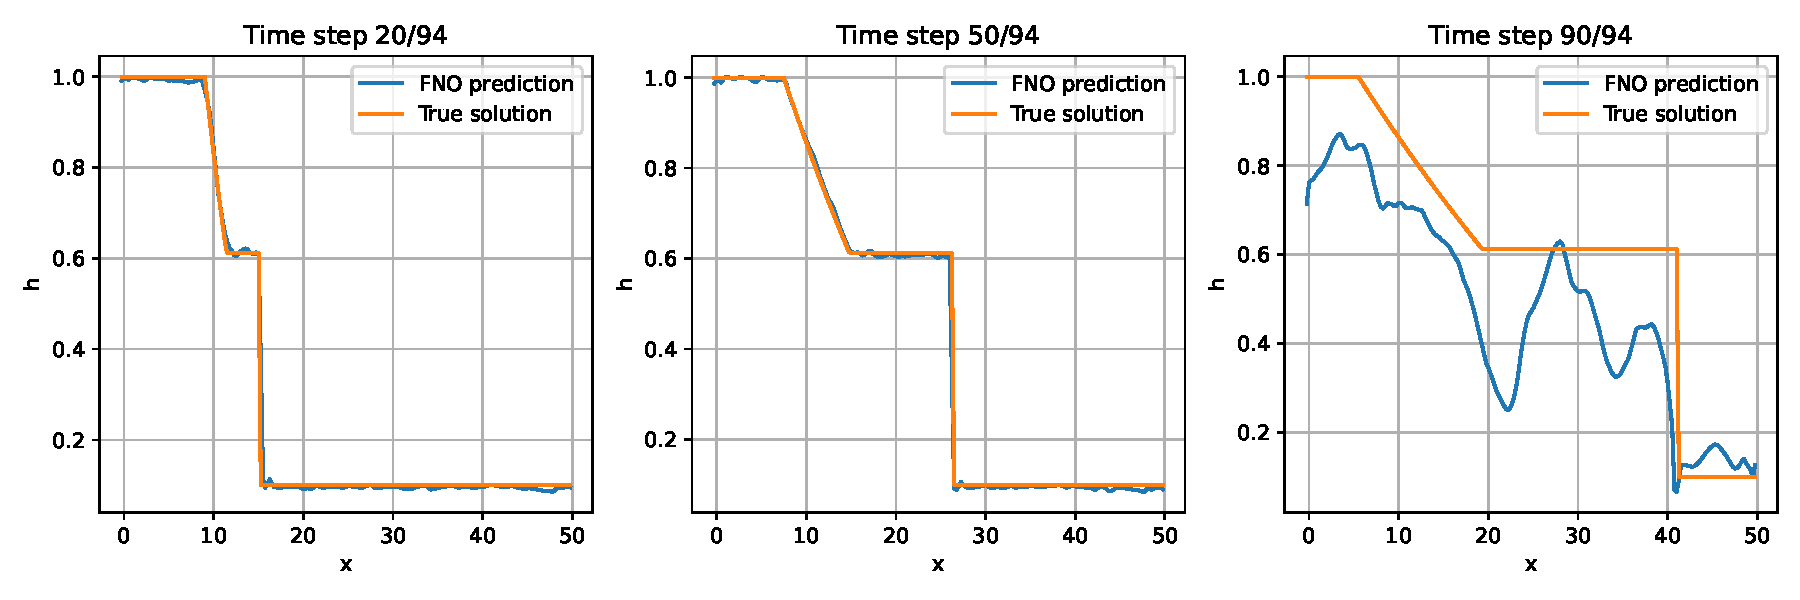
\includegraphics[width=0.9\textwidth]{C:/Users/Matteo/Shallow-Water-Equations/plots/torotest1_predictions_time_steps.pdf}
    \caption{FNO Toro test 1 predictions timesteps.}\label{fig:FNO_Toro_test1_predictions_time_steps}
\end{figure}


\begin{figure}[H]
    \centering
    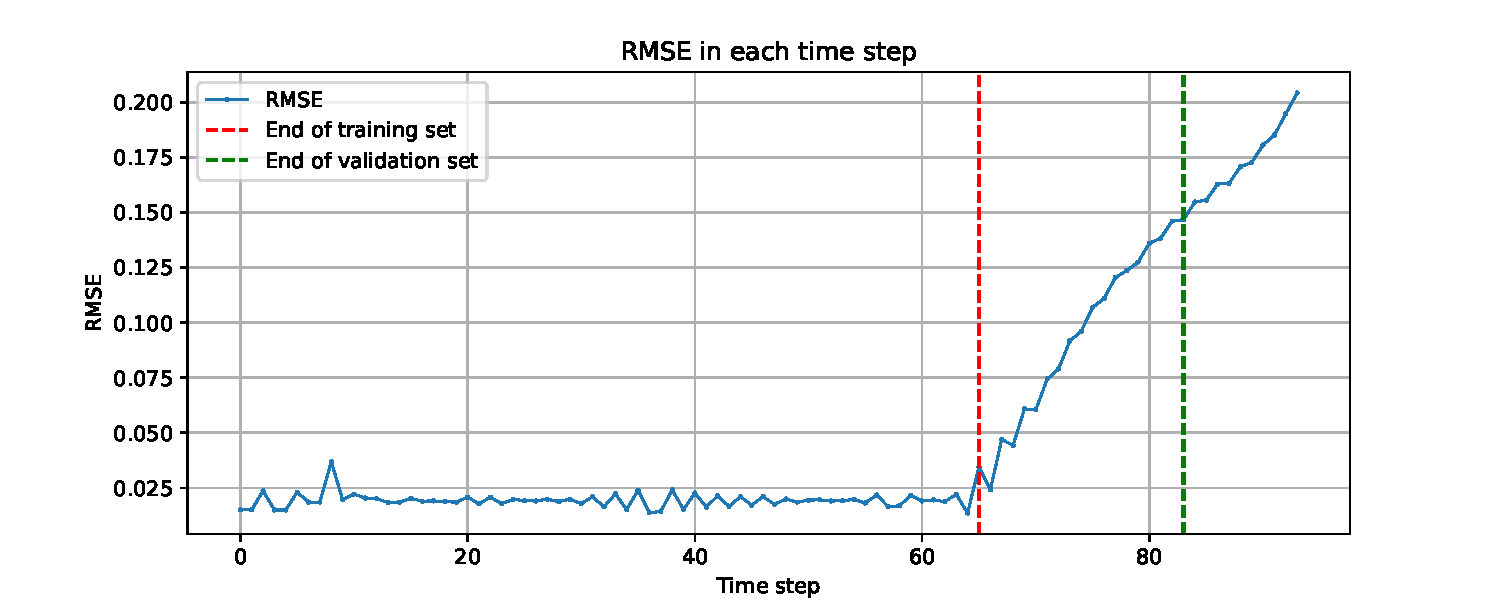
\includegraphics[width=0.7\textwidth]{C:/Users/Matteo/Shallow-Water-Equations/plots/torotest1_RMSE.pdf}
    \caption{FNO Toro test 1 predictions RMSE.}\label{fig:FNO_Toro_test1_rmse}
\end{figure}


